\begin{figure}[t]
\centering
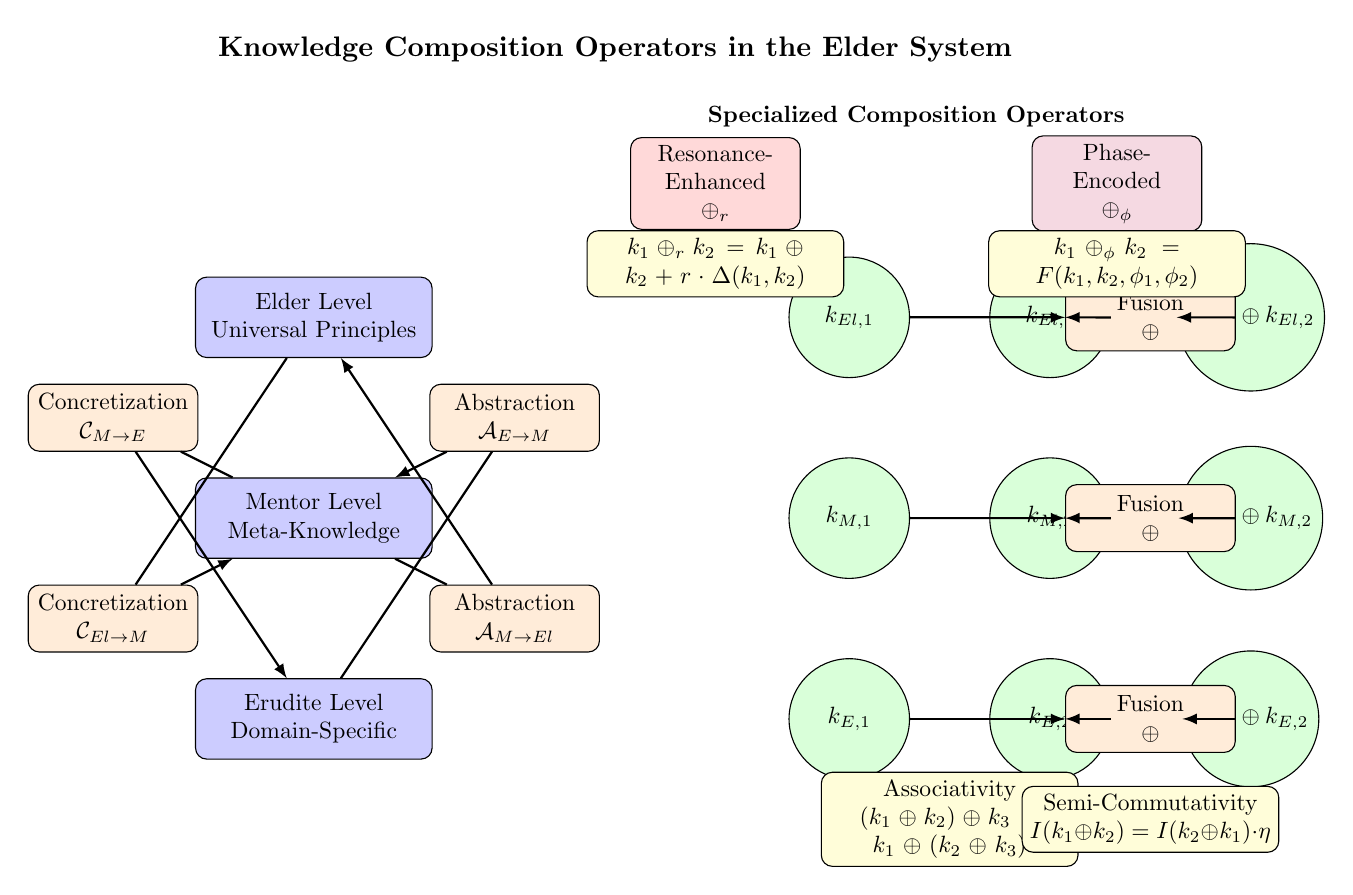
\begin{tikzpicture}[scale=0.85, transform shape]
    % Define styles
    \tikzset{
        level/.style={
            draw,
            fill=blue!20,
            rounded corners,
            minimum width=3.5cm,
            minimum height=1.2cm,
            text width=3.3cm,
            align=center
        },
        knowledge/.style={
            draw,
            fill=green!15,
            circle,
            minimum size=1.8cm,
            align=center
        },
        operator/.style={
            draw,
            fill=orange!15,
            rectangle,
            rounded corners,
            minimum width=2.5cm,
            minimum height=1cm,
            text width=2.3cm,
            align=center
        },
        property/.style={
            draw,
            fill=yellow!15,
            rounded corners,
            minimum width=3.8cm,
            minimum height=0.8cm,
            text width=3.6cm,
            align=center
        },
        arrow/.style={
            ->,
            thick,
            >=latex
        }
    }
    
    % Hierarchical levels
    \node[level] (elder) at (0,6) {Elder Level\\Universal Principles};
    \node[level] (mentor) at (0,3) {Mentor Level\\Meta-Knowledge};
    \node[level] (erudite) at (0,0) {Erudite Level\\Domain-Specific};
    
    % Vertical operators
    \node[operator] (abst1) at (3,4.5) {Abstraction\\$\mathcal{A}_{E \rightarrow M}$};
    \node[operator] (abst2) at (3,1.5) {Abstraction\\$\mathcal{A}_{M \rightarrow El}$};
    
    \node[operator] (conc1) at (-3,4.5) {Concretization\\$\mathcal{C}_{M \rightarrow E}$};
    \node[operator] (conc2) at (-3,1.5) {Concretization\\$\mathcal{C}_{El \rightarrow M}$};
    
    % Vertical connections
    \draw[arrow] (erudite) -- (abst1) -- (mentor);
    \draw[arrow] (mentor) -- (abst2) -- (elder);
    \draw[arrow] (mentor) -- (conc1) -- (erudite);
    \draw[arrow] (elder) -- (conc2) -- (mentor);
    
    % Horizontal operators (represented at each level)
    \begin{scope}[shift={(8,0)}]
        % Erudite level
        \node[knowledge] (ke1) at (0,0) {$k_{E,1}$};
        \node[knowledge] (ke2) at (3,0) {$k_{E,2}$};
        \node[knowledge] (ke_fused) at (6,0) {$k_{E,1} \oplus k_{E,2}$};
        
        \node[operator] (fusion_e) at (4.5,0) {Fusion\\$\oplus$};
        
        \draw[arrow] (ke1) -- (3,0) |- (fusion_e);
        \draw[arrow] (ke2) -- (fusion_e);
        \draw[arrow] (fusion_e) -- (ke_fused);
        
        % Properties
        \node[property] at (1.5,-1.5) {Associativity\\$(k_1 \oplus k_2) \oplus k_3 = k_1 \oplus (k_2 \oplus k_3)$};
        \node[property] at (4.5,-1.5) {Semi-Commutativity\\$I(k_1 \oplus k_2) = I(k_2 \oplus k_1) \cdot \eta$};
        
        % Mentor level
        \node[knowledge] (km1) at (0,3) {$k_{M,1}$};
        \node[knowledge] (km2) at (3,3) {$k_{M,2}$};
        \node[knowledge] (km_fused) at (6,3) {$k_{M,1} \oplus k_{M,2}$};
        
        \node[operator] (fusion_m) at (4.5,3) {Fusion\\$\oplus$};
        
        \draw[arrow] (km1) -- (3,3) |- (fusion_m);
        \draw[arrow] (km2) -- (fusion_m);
        \draw[arrow] (fusion_m) -- (km_fused);
        
        % Elder level
        \node[knowledge] (kel1) at (0,6) {$k_{El,1}$};
        \node[knowledge] (kel2) at (3,6) {$k_{El,2}$};
        \node[knowledge] (kel_fused) at (6,6) {$k_{El,1} \oplus k_{El,2}$};
        
        \node[operator] (fusion_el) at (4.5,6) {Fusion\\$\oplus$};
        
        \draw[arrow] (kel1) -- (3,6) |- (fusion_el);
        \draw[arrow] (kel2) -- (fusion_el);
        \draw[arrow] (fusion_el) -- (kel_fused);
    \end{scope}
    
    % Special operators
    \begin{scope}[shift={(9,9)}]
        \node[align=center, font=\bfseries] at (0,0) {Specialized Composition Operators};
        
        % Resonance-enhanced fusion
        \node[operator, fill=red!15] (res_fusion) at (-3,-1) {Resonance-Enhanced\\$\oplus_r$};
        \node[property] at (-3,-2.2) {$k_1 \oplus_r k_2 = k_1 \oplus k_2 + r \cdot \Delta(k_1, k_2)$};
        
        % Phase-encoded fusion
        \node[operator, fill=purple!15] (phase_fusion) at (3,-1) {Phase-Encoded\\$\oplus_\phi$};
        \node[property] at (3,-2.2) {$k_1 \oplus_\phi k_2 = F(k_1, k_2, \phi_1, \phi_2)$};
    \end{scope}
    
    % Title
    \node[align=center, font=\bfseries, scale=1.2] at (4.5,10) {Knowledge Composition Operators in the Elder System};
    
\end{tikzpicture}
\caption{Knowledge composition operators in the Elder system. Vertical operators transfer knowledge between hierarchical levels: abstraction ($\mathcal{A}$) maps knowledge from lower to higher levels through generalization, while concretization ($\mathcal{C}$) maps knowledge from higher to lower levels through specialization. Horizontal operators combine knowledge within the same level, including fusion ($\oplus$), intersection ($\cap$), and difference ($\setminus$), with properties like associativity and semi-commutativity. Specialized operators include resonance-enhanced fusion ($\oplus_r$), which leverages resonance strength $r$ to generate emergent knowledge $\Delta(k_1, k_2)$, and phase-encoded fusion ($\oplus_\phi$), which incorporates phase information for enhanced composition. These operators form an algebraic framework for understanding how knowledge composes across the Elder system's hierarchical structure, enabling efficient abstraction, transfer, and recombination.}
\label{fig:composition_operators}
\end{figure}